% Created 2022-03-16 mié 17:36
% Intended LaTeX compiler: pdflatex
\documentclass[twoside]{article}
\usepackage[utf8]{inputenc}
\usepackage[T1]{fontenc}
\usepackage{graphicx}
\usepackage{grffile}
\usepackage{longtable}
\usepackage{wrapfig}
\usepackage{rotating}
\usepackage[normalem]{ulem}
\usepackage{amsmath}
\usepackage{textcomp}
\usepackage{amssymb}
\usepackage{capt-of}
\usepackage{hyperref}
\renewcommand\maketitle{\begin{titlepage}%
\begin{center}
       \vspace*{1cm}

       \textbf{Modelo de literariedad usando redes semánticas y n-gramas}

       \vspace{0.5cm}
        
            
       \vspace{1.5cm}

       \textbf{Jonatan Ahumada Fernández}

       \vfill
            
       Tesis para el título de Ingeniería de Sistemas
            
       \vspace{0.8cm}
     
       \includegraphics[width=0.4\textwidth]{university}
            
       Facultad de Matemáticas E Ingeniería\\
       Fundación Universitaria Konrad Lorenz\\
       Bogotá, Colombia\\
       2022
            
   \end{center}\end{titlepage}%
}

\usepackage{longtable}
\author{Jonatan Ahumada Fernández}
\date{\today}
\title{Modelo de literariedad usando redes semánticas y n-gramas}
\hypersetup{
 pdfauthor={Jonatan Ahumada Fernández},
 pdftitle={Modelo de literariedad usando redes semánticas y n-gramas},
 pdfkeywords={},
 pdfsubject={},
 pdfcreator={Emacs 27.2 (Org mode 9.4.4)}, 
 pdflang={English}}
\begin{document}

\maketitle
\tableofcontents

\section{FORMULACIÓN DEL PROBLEMA}
\label{sec:org1ad63c3}
\subsection{Introducción}
\label{sec:orga0685e3}

¿Qué constituye la esencia de un texto? ¿Qué diferencia un texto
considerado 'literario' de aquél que no lo es? Esta pregunta se ha
planteado en áreas como los estudios literarios y la lingüística
\cite{eijembaum2010teoria}. Particularmente, la escuela denominada
'formalismo ruso' planteó que el objeto de estudio de la literatura,
no \emph{podría} ser la belleza, la relevancia histórica o el valor
pragmático de un texto. Más bien, su objeto de estudio \emph{debe} recaer
en un aspecto más 'objetivo': su \emph{literariedad}.  Como su nombre
sugiere, los formalistas se abocaron a formular una definición
'objetiva' y 'concreta' del fenómeno literario y adoptaron los --en
ese entonces-- modernos métodos de la buyente disciplina de la
linguística.

Siendo este el caso, ¿no es, por consiguiente, factible que un
autómata pueda medir y presentar tales características presuntamente
formales con las actuales herramientas informáticas? ¿Cómo se podría
traducir la noción de \emph{literariedad} a un algoritmo que pueda ejecutar
una máquina?


\subsection{Planteamiento del problema}
\label{sec:orgfac9285}
Roman Jakobson propone que la \emph{literariedad} de un texto está dada por
dos componentes de lenguaje: la diacronía y la sincronía. Estos
elementos fueron expandidos de la teoría linguística de Saussure.
Más tarde, puestos en el contexto del análisis de la poesía,
Jakobson renombró esos dos ejes como \emph{metáfora} y \emph{metonímia}, en su texto
"Linguística y poética". 



\begin{figure}[htbp]
\centering
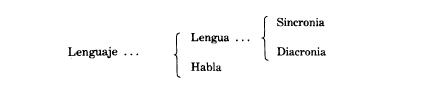
\includegraphics[width=.9\linewidth]{./assets/clasificacion_saussure.png}
\caption{Distinción entre sincronía y diacronía}
\end{figure}

¿Es posible  modelar algorítmicamente  tales conceptos? Según
Jakobson, en el estudio de la \emph{literariedad} se omite el factor emisor
y factor receptor. Tan solo se centra en el mensaje. Representado
 únicamente a través de un \emph{medio} particular: en este caso, la palabra escrita.
Es, por lo tanto,  \emph{factible} que un autómata pueda medir y presentar tales
características. 

\begin{figure}[htbp]
\centering
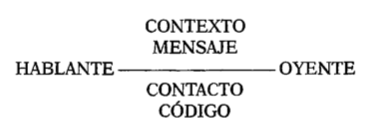
\includegraphics[width=.9\linewidth]{./assets/factores_comunicacion.png}
\caption{Factores de comunicación de Roman Jakobson \cite{jakobson1981linguistica}}
\end{figure}

Saussure ofrece ya un modelo cualitativo muy bien esbozado en teoría,
que es el que luego Jakobson utilizará para definir la literariaded.
Sin embargo, aunque existe un planteamiento cualitativo del problema,
no se halló en la bibliografía consultada un modelo computacional que
modelara el concepto y lo implementara. 

\begin{figure}[htbp]
\centering
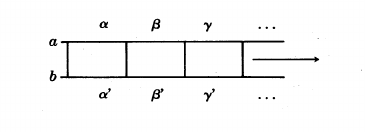
\includegraphics[width=.9\linewidth]{./assets/delimitacion_saussure.png}
\caption{Modelo cualitativo inicial expuesto por Ferdinand De Saussure tomado de \cite{eijembaum2010teoria}}
\end{figure}

Preliminarmente, se puede observar que el modelo de Saussure se
fundamenta en una estructura bastante familiar en la computación: la
secuencia \cite{alonso1945curso}. Así, el objetivo de este trabajo es modelar e implementar el
modelo de \emph{literariedad} de Roman Jakobson utilizando redes semánticas
y n-gramas.


\subsection{Justificacón}
\label{sec:org512600f}

Si bien existen infinitas operaciones realizables sobre un texto
computarizado, hay pocas que tengan un enfoque humanístico, sea
este linguístico, literario o estético. Este
enfoque busca generar una mayor comprensión del fenómeno literario,
en contraposición a los enfoques 'típicos' --y hoy en día
indispensables-- de procesamiento de lenguaje: extracción de
información, clasificación con base a un modelo predictivo, entre
muchos otros \cite{gelbukh2004}.

Más aún, dentro de este subcunjunto reducido, pocos están guiados por
aquello que Gelbuhk llama 'la ciencia fundamental'. A saber, la
linguística. En otras palabras, hay un vacío en el campo de la
linguística computacional en lo que se refiere a modelos que procuran
cuantificar esta perspectiva.

Tal vacío genera que el estudio académico de la literatura no pueda
sustentarse en datos 'duros' o ,por lo menos, cuantitativos propias
del método científico. Por otro lado, los diversas y posibles formas
de calcular la 'creatividad', la 'rima' o la 'belleza' de un texto,
propuesto por otros investigadores, pueden considerarse casuísticos,
acoplados a las objetivos y circunstancias de cada investigación en
particular, desde la perspectiva de la linguística general.

Así, se necesita un modelo de la \emph{literariedad} que exprese
concretamente la metáfora y la metonimia. Bien sea para ampliar las
aplicaciones de la linguistica computacional o para someter a
escrutinio los planteamientos de la teoría.

En esta investigación se formulará y evaluará un modelo para obtener
una medida cuantitativa para el concepto de \emph{literariedad} de Roman
Jakobson utilizando redes semánticas y n-gramas. De este modo, la
presente investigación respondería a la pregunta ¿Cómo medir
computarizadamente la \emph{literariedad} de un texto según el marco de la
lingüística de Jakobson?

\subsubsection{\textbf{Palabras clave:}}
\label{sec:orgddeb870}
NLP, computational linguistics, literariness,literary theory, poetics, theory of formal method

\subsubsection{\textbf{Área de conocimiento:}}
\label{sec:org8268724}

Lingüística computacional

\subsection{Alcances y delimitaciones:}
\label{sec:orga6fd7e7}

Para computar una métrica de \emph{literariedad} será necesario comparar
un \emph{corpus objetivo} con respecto a un \emph{corpus de referencia,} este
último representará el ‘uso corriente de la lengua'. La primera
limitación de este trabajo es que no se compilará un corpus propio, sino
que partirá de los de acceso libre. La mayoría de estos se encuentran en
inglés. Por este motivo, el corpus de referencia más a la mano es
WordNet, que al ser una ontología ya contiene las anotaciones necesarias
para mi objetivo. A saber, una lista de sinónimos por palabras. Por otro
lado, el corpus objetivo no tiene que estar anotado (utilizaré un
PlainTextCorpus), pero de algún modo tiene que ser razonable su
comparación con el corpus objetivo. Por ejemplo, los resultados del
modelo serían muy difíciles de evaluar si la relación entre corpus
objetivo y de referencia sobrepasa los 2 siglos, dada la naturaleza
fluida de la lengua.

La segunda limitación concierne a la formulación de los algoritmos en sí
mismos. Me limitaré a formular los modelos más naive posibles. Por
ejemplo, (retomando el ejemplo previo) dada una palabra se considerará
un sinónimo todas las palabras listadas como tal en el corpus de
referencia, sin considerar los sub-problemas que esto podría conllevar.

En general, el alcance de este proyecto es formular e implementar un
modelo general que muestre cómo sería viable implementar el concepto de
\emph{literariedad}, sin ahondar en los detalles que se desprenden de cada
fase del flujo de NLP (por ejemplo, ¿cómo tokenizar?, ¿Qué peso tendrían
las diferentes partes de una oración en el computo final, etc).

\section{OBJETIVO GENERAL}
\label{sec:org6f6c102}
Diseñar e implementar un modelo que, dado un corpus de texto, produzca
indicadores para el concepto de \emph{literariedad} que plantea Roman Jakobson.

\section{OBJETIVOS ESPECÍFICOS}
\label{sec:org09ff8e6}

\begin{enumerate}
\item Construir el corpus necesario para representar el \emph{eje diacrónico}
\item Diseñar e implementar el algoritmo para calcular la \emph{metáfora} sobre un corpus
\item Diseñar e implementar algoritmo para calcular la \emph{metonimia} sobre un corpus
\item Seleccionar y unir los textos que serán procesados (corpus objetivo) por el algoritmo
\item Correr el algoritmo sobre los corpus objetivo
\item Evaluar el algoritmo de manera cuantitativa y cualitativa
\end{enumerate}

\section{MARCO TEÓRICO}
\label{sec:org6764820}

\subsection{Literariedad}
\label{sec:org16d1847}


La \emph{literariedad} es, según Jakobson, la cualidad de un objeto
literario en cuanto tal. Por lo tanto, la \emph{literariedad} no depende de
ningún factor extrínseco, como su emisor, su valor histórico, las
ventas de tal o cual libro, las citaciones, etc. La \emph{literariedad} se
da exclusivamente por atributos propios del fenómeno del lenguaje.

Para analizar la \emph{literariedad}, se deben analizar las dos operaciones
más básicas de la conducta verbal: \emph{la selección} y \emph{la combinación.}


\subsubsection{Selección (ver linguística sincrónica):}
\label{sec:org3f6914f}

La selección estudia qué palabra selecciona un hablante entre las
palabras existentes de la lengua, más o menos similares y hasta
cierto punto equivalentes. La selección se basa en la sinonimia o
antonimia de una palabra. En otros términos, en su semántica.


\subsubsection{Combinación (ver linguística diacrónica):}
\label{sec:org7a41a83}

La combinación estudia el "entramado de la secuencia" de un
mensaje. Es decir, el mensaje considerado como una secuencia
temporal y/o ordenada de palabras. La combinación se basa en la
proximidad o, en otras palabras, en la relación de una palabra con
la que la sucede o antecede en un mensaje.



\subsection{Poética}
\label{sec:orgfdd0533}
La poética procura responder a la pregunta de ¿qué hace que un
mensaje (verbal o de otra naturaleza) sea una obra de arte? Lidia
principalmente con cuestiones estéticas del lenguaje. Sin embargo,
para hacer un analisis exhaustivo, la poética debe hacer uso de la
linguística, puesto que esta última estudia el lenguaje en todo su
conjunto. La \emph{literariedad} podría, entonces, considerarse un
concepto enmarcado en la poética, porque se preguntá qué hace que
un texto sea literario y por qué es distinto de otro que no lo es.

\subsection{Linguística}
\label{sec:orgee87f95}

La lingüística es la ciencia que estudia el lenguaje.
Tradicionalmente, esta ciencia se subdivide en las ramas de fonética,
fonología, morfología, sintaxis, semántica y pragmática.

La lingüística es un campo de estudio interdisciplinar e involucra
disciplinas heterogéneas como la lógica y la neurolingüistica. Sin
embargo, se considera que hay un núcleo común llamado \emph{linguística
general}.

\subsubsection{Lingüística General:}
\label{sec:orgb6e66bc}

Se conoce como lingüística general al paradigma lingüístico
establecido por Ferdinand De Saussure, también llamado \emph{modelo
diferencial del lenguaje}.

El modelo diferencial se caracteriza porque propone dos ejes
principales existentes en todo fenómeno lingüístico: el \emph{eje de
sincronía} y el \emph{eje de diacronía}.

Estos dos ejes son la base de lo que Jakobson considera \emph{selección} y
\emph{combinación}.


\subsubsection{Linguística sincrónica}
\label{sec:orgecb6776}

La linguística sincrónica se ocupa de las
operaciones que realiza un hablante, sean lógicas o psicológicas,
para formar un sistema linguístico. En el
marco de esta investigación el \emph{eje sincrónico} se referirá a las
posibles palabras que un hablante pudo haber seleccionado para
expresar una misma idea. Por ejemplo, para referirse a un
niño, un hablante puede utilizar la las palabras "niño", "chico",
"jovencito", o "párvulo".


\subsubsection{Linguística diacrónica}
\label{sec:org41323d9}

La linguística diacrónica estudia los cambios sucesivos en el
lenguaje, producidos por la actividad constante del \emph{eje
sincrónico}. En la perspectiva de Jakobson, un \emph{mensaje} tiene en
sí mismo un eje diacrónico. Tal eje mide la similaridad entre cada
término del mensaje entindido como secuencia. Un ejemplo se puede
apreciar en la oracion "I like Ike". An esta se evidencia una
repetición de sonidos similares: [ay layk ayk]. La similaridad, no
está dada por el significado, sino que aquí se proyecta a lo largo
del tiempo:"(\ldots{}) para decirlo de un modo más técnico: todo
secuencia es un símil."

\subsection{Lenguaje}
\label{sec:org60b0751}
En términos simples, el lenguaje es la facultad de formular y
comprender signos o símbolos, ya sean hablados, escritos,
imágenes, etc.  En otros términos, el lenguaje es una capacidad
general. Sin embargo, para Saussure, la lengua tiene una
característica doble: que es al mismo tiempo un sistema
establecido y la constante evolución de tal sistema. Estos dos
componentes son la \emph{lengua} y el \emph{habla}.

\subsubsection{Lengua}
\label{sec:org7e5acf6}

La lengua (\emph{langue}) es uno de los dos componentes del
\emph{lenguaje}.  La lengua es fenómeno social y se equipara a una
\emph{cristalización} o un producto de la suma de asociaciones entre
conceptos e imagenes acústicas en la mente de los hablantes. Por
ejemplo, la lengua es lo que permite que dos hablantes bogotanos
puedan asociar en su mente el sonido de la palabra "chino" con el
concepto de "niño" o "infante", mientras que en otras partes del
mundo hispanohablante no existe tal asociación común.
En términos simples, la lengua es un entendimiento compartido de
lo que significan las palabras. La contraparte de la lengua,
es el habla. 

\subsubsection{Habla}
\label{sec:org0daa3d1}
El habla (\emph{parole}) es uno de los dos componentes del
\emph{lenguaje}. El habla es el uso individual de la lengua.
Evidentemente, cuando un individuo habla puede modificar
la lengua a su antojo, porque posee la facultad del
lenguaje y jamás meramente repite el consenso de la lengua.
Como consecuencia de esto, la lengua está continuamente
siendo transformada por el habla. En términos simples,
la suma de los actos individuales de comunicacion lentamente
terminan por transformar el consenso social sobre cómo
hablar.  Por este motivo la linguística debe tener una
perspectiva doble: \emph{diacrónica} y \emph{sincrónica}.


\subsection{Lingüística Computacional}
\label{sec:orgf378e3d}

Es la intersección entre la computación y la lingüística. Por lo
general, se preocupa acerca de cómo procesar automáticamente el
lenguaje material, para lo cual genera modelos lingüísticos sobre los
que luego se pueden definir operaciones comunes \cite{gelbukh2004}.


La lingüística computacional es en sí misma un campo amplio y
heterogéneo, pero en términos de este trabajo, me limitaré a señalar
una herramienta:

\subsubsection{NLTK}
\label{sec:orgd7143ae}

El Natural Language Toolkit (NLTK) es un módulo de Python que
ofrece una interfaz para tareas comunes en la lingüística
computacional. La ventaja principal de NLTK es que se considera a
sí mismo un \emph{toolkit}. Esto significa que no impone una estructura
de procesamiento definida a la vez que ofrece un extenso abanico de
herramientas, tales como: tokenizacion, filtros, generación de
n-gramas, análisis sintáctico de oraciones, entre otras.

\subsubsection{Corpus}
\label{sec:org37fc776}


Un corpus es una colección de textos auténticos que pueden ser
leídos por una máquina. Estos pueden estructurarse de muchas
formas, dependiendo de los objetivos de la investigación
\cite{indurkhya2010handbook}. Por ejemplo, pueden ser aislados (una
colección arbitraria), categorizados (una colección escogida según
algún criterio), temporales (una colección organizada
cronológicamente) o solapados (un documento puede pertenecer a
varias colecciones) \cite{bird2009natural}. Además, el formato del
corpus varía significativamente de acuerdo al objeto de la
investigación. Por ejemplo, si se desea hacer un análisis
sintáctico (de la estructura de una oración), se debe hacer un
corpus anotado con POS (Part Of Speech tag); para hacer un análisis
pragmático se utiliza una anotación pragmática, etc.

\begin{figure}[htbp]
\centering
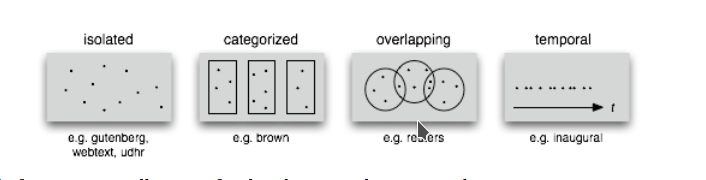
\includegraphics[width=.9\linewidth]{./assets/estructuras_de_corpus.png}
\caption{Diferentes estructuras de corpus}
\end{figure}

\section{MARCO REFERENCIAL}
\label{sec:org4dfbaa0}

El trabajo de Delmonte \cite{delmonte2013computing} presenta a
SPARSAR, un sistema para calcular automáticamente el estilo de la
poesía. SPARSAR funciona sobre sistemas previos del mismo autor, como,
por ejemplo, un analizador semántico \cite{delmonte2005venses}.
Delmonte tiene una larga trayectoria en el modelamiento de conceptos
lingüísticos "difíciles", como la prosodia y la rima en términos
cuantitativos.

El aporte principal de Delmonte fue su innovación al momento de aplicar
herramientas comunes de NLP (tokenizadores, splitters y NER) con el fin
de analizar aspectos estilísticos de un texto. Los modelos de Delmonte
son muy cercanos a la teoría lingüística y propone soluciones a aspectos
complejos del análisis lingüístico. Esta proximidad me llevo a
plantearme la pregunta ¿qué otros aspectos del lenguaje valdría la pena
modelar que aún no hayan sido abordados desde una perspectiva
computacional? Así mismo, Delmonte reporta que hay pocos trabajos en el
área con este mismo enfoque. Esta fue una inspiración para explorar más
en el tema y ofrecer un enfoque distinto, tal como él lo hizo.

Sin embargo, Delmonte no revela detalles de implementación de sus sis-
temas en los artículos revisados. Además, sus sistemas tienen una
alcance mucho mayor que el dispuesto para este trabajo, por lo que para
mayores detalles tuve que referirme a otros trabajos.

El trabajo de \cite{zuniga2017automatic} establece una métrica para
medir el grado de creatividad en la poesía, basándose en qué tanto de
la rima se conserva en la traducción de un poema con respecto al
original. Tomé de Zuñiga la idea de establecer una métrica para un
aspecto tradicionalmente cualitativo (la creatividad). Lo que
diferencia este trabajo del de Delmonte, es su aproximación
matemática. Particularmente, Zuñiga ofreció una forma naive de
calcular similitud en rima, sin necesidad de recurrir a construcciones
que requieren de recursos léxicos complejos como una ontología para
fonemas, etc.

Por último, el trabajo de \cite{kaplan2006computational} es una tesis
de pregrado sobre el cálculo del estilo de la poesía desde una
perspectiva estadística. Kaplan fue una inspiración para Delmonte, por
lo tanto debía formar parte de mi revisión bibliográfica. Kaplan
formuló un modelo que media 84 métricas distintas para cada documento,
luego transformó el modelo de 84 métricas para visualizarlo en un
espacio 3D y poder comparar distintas obras literarias. Esto inspiró
mi idea inicial de obtener una métrica más general para analizar un
texto, que no tenga que recurrir un trabajo de compilación de métricas
existentes, como lo hizo Kaplan. Tal métrica debería estar sustentada
en conceptos linguísticos, para lo cual recurre en los conceptos
presentados en el marco teórico.

\section{DISEÑO METODOLÓGICO}
\label{sec:org0ee8488}
El diseño metodológico seguirá --a grandes rasgos-- los pasos de la
metodología CRISP-DM, que se considera un estándar \emph{de facto} para
proyectos de minería de datos. Esta metodología ayudará organizar
el proceso de mi investigación, que vá desde el acceso a los corpus
(los datos disponibles) hasta el despliegue (la visualización de
los resultados).

\subsection{Entendimiento del negocio}
\label{sec:orgf7ba487}

El resultado tangible del modelo de literariedad propuesto son dos
métricas cuantitativas: \emph{metáfora} y \emph{metonímia}.  Estas métricas
juntas constituiran una representación 'objetiva' del concepto
cualitativo de \emph{literariedad}.

\begin{figure}[htbp]
\centering
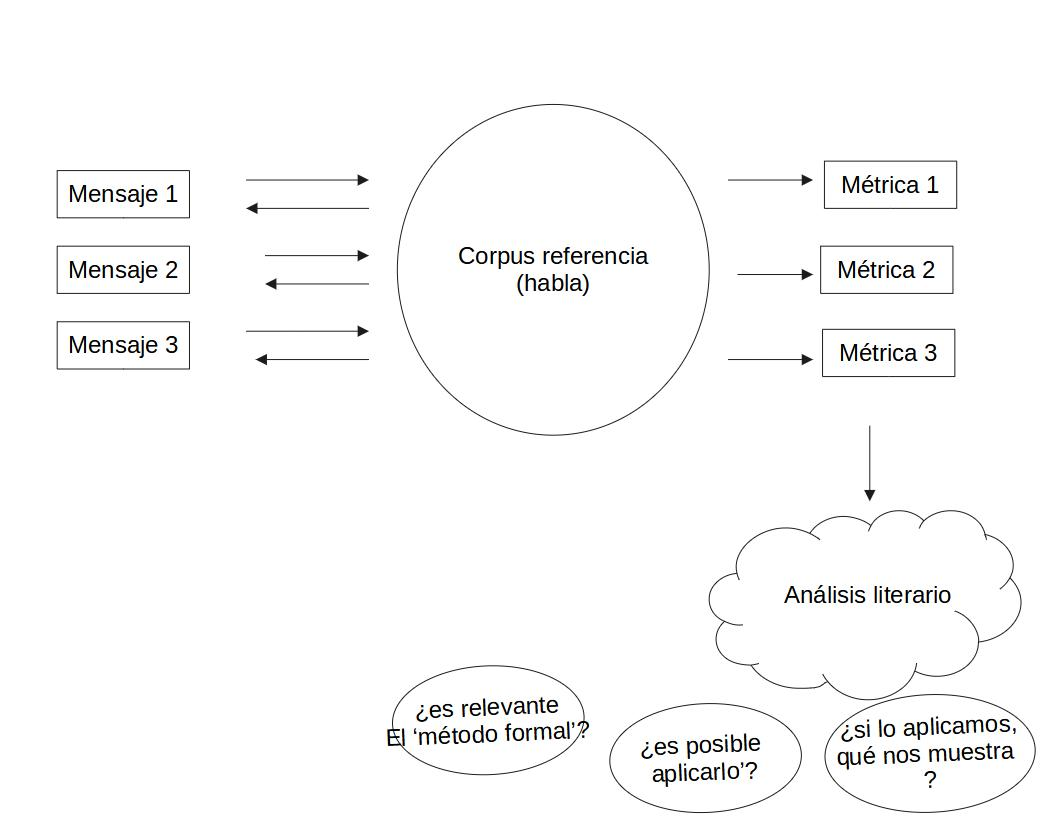
\includegraphics[width=.9\linewidth]{./assets/posibles_usos.jpg}
\caption{\label{fig:posibles_usos}Entradas y salidas del algoritmo}
\end{figure}


¿Cuál sería el beneficio de obtener este resultado? Se podría
comparar las métricas de n mensajes cualesquiera y tener una
medida objetiva con las cuales compararlas. Algunos casos de uso
posible serían:

\begin{itemize}
\item determinar si un mensaje que yo he escrito es más metáforico o
metonímico que otro.

\item determinar si un mensajes de una misma categoria (por ejemplo,
del mismo autor, o del mismo género) tienen medidas de métadora
y metonímia similares.

\item correr grandes grupos de mensajes, por ejemplo, 'poemas de la
escuela simbolistas' y compararlo con 'poemas realistas' y
verificar si hay o no una diferencia sustancial desde el punto
de vista linguístico .
\end{itemize}

Como se puede apreciar (ref:fig:posibles\textsubscript{usos}), las aplicaciones
del modelo en principio supondrían un factor adicional para ser
considerado para el estudio literario, cuya naturaleza es
cualitativa. Sin embargo, si el modelo demuestra ser efectivo,
podría llegar a ser una medida de similitud para un texto, lo que
implicaría que se podría clasificar un texto con base en su
metáfora y metonímia,


\subsection{Entendimiento de los datos}
\label{sec:orgb61eff9}

En esta sección, se enumeraran las distintas fuentes de datos,
que en este caso vendrían a ser los diferentes tipos de corpus.


\subsubsection{El corpus de referencia}
\label{sec:orgb00e409}

El corpus de referencia es un compendio de muestras
que terminará por representar un consenso sobre
el uso de la \emph{lengua}. Su correlación teórica
es el eje de diacronía y cumple la función de
cristalizar una lengua en un lugar y un tiempo establecido.
A nivel de implementación, se trata de un cadena muy larga
compuesto de muestras seleccionadas según criterios aptos
(ver sección sobre preparación de los datos).




\subsubsection{El corpus objetivo}
\label{sec:orga36e874}

El corpus objetivo serán los mensajes sobre los cuales se
computarán las dos medidas de \emph{metáfora} y \emph{metonimia}.
Su correlativo teórico es el \emph{habla} y son los
textos que el usuario final del final del sistema desea
someter a análisis. A nivel de implementación, cada mensaje
es una cadena (que corresponde a un documento real), pero
en su totalidad el corpus objetivo es mucho más pequeño
que el corpus de referencia, del mismo modo en que una
persona que profiere una oración utiliza un subconjunto
mucho más pequeño de la lengua a la que pertenece.  

\subsubsection{La red semántica}
\label{sec:org64a11bd}

La red semántica es un tipo de corpus particular que no solamente
consta de palabras anotadas, como el de Brown, sino que vincula
las palabras por su relación conceptual con otras palabras. La
red semántica correspondería a la facultad de asociar conceptos
con las "imágenes acústicas" (las palabras) de Saussure. En esta
investigación, la red semántica se utilizará para obtener
sínonimos de palabras, que representarán conceptos. Tal red
no será implementada, sino que será un servicio utilizado por
el algoritmo. 



\subsubsection{Resumen de entendimiento de los datos}
\label{sec:org036bc7c}
\begin{figure}[htbp]
\centering
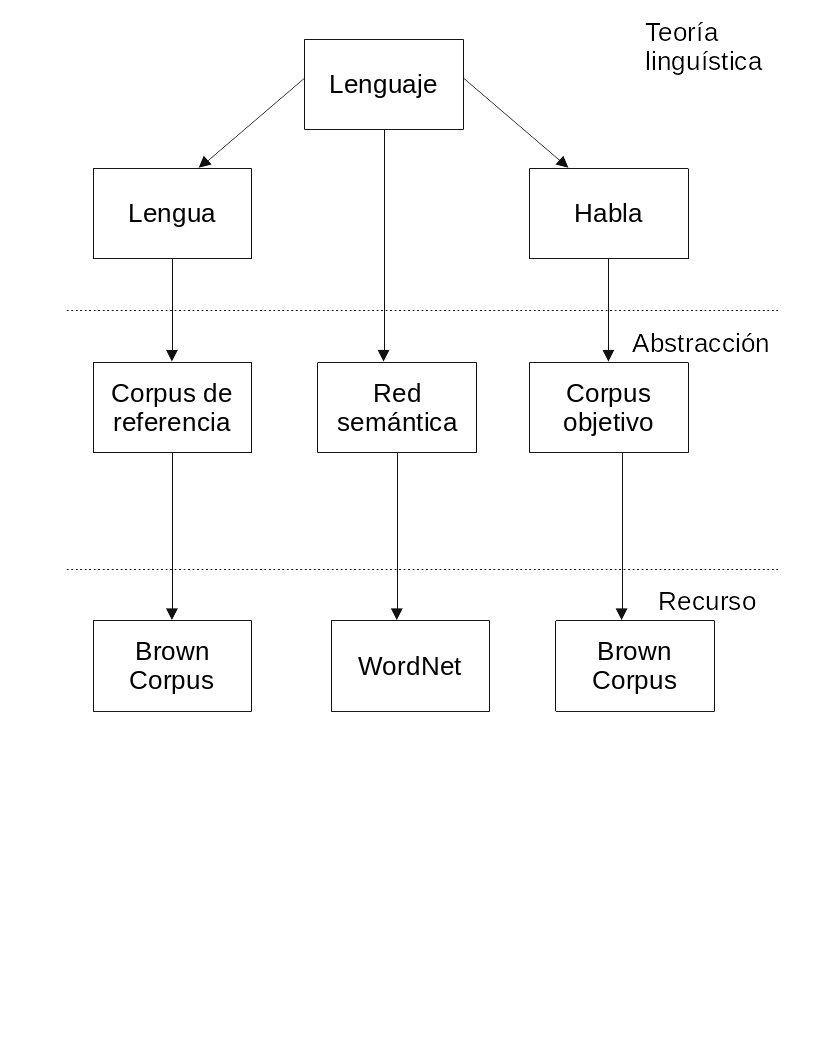
\includegraphics[width=.9\linewidth]{./assets/entendimiento_de_los_datos.png}
\caption{Resumen de las fuentes de datos utilizadas para cada concepto}
\end{figure}


\subsection{Preparación de los datos}
\label{sec:org6078752}
La tarea de preparación de los datos consitirá principalmente en
seleccionar los distintos tipos de corpus de manera significativa
y coherente.  A continuación, describiré cómo se conformaron los
corpus y qué criterios se utilizaron.

\subsubsection{Corpus de referencia}
\label{sec:org974c2b8}
El corpus de referencia representa la \emph{lengua} (\emph{langue}). Por lo
tanto debe estar compuesto de una muestra de textos
comparativamente mucho más grande los mensajes individuales que
serán contrastados con este. ¿Cómo construir un corpus tal?

En primer lugar, se descartó la idea de modelar la \emph{lengua} en su
totalidad, pues como lo indica la teoría linguística, esta tarea
es imposible puesto que esta se encuentra en constante
cambio. Así, el primer criterio para construcción del corpus fue
restringirlo diacrónicamente al espacio de un año y a un idioma
específico.

El siguiente criterio fue armar un corpus \emph{balanceado}. Es decir,
el corpus de referencia no puede estar compuesto de muestras de
un mismo tipo (un estilo, un género, un autor), porque esto
sesgaría la comparación de el corpus objetivo con respecto a
este. Así, se optó por partir de un corpus \emph{categorizado} y tomar
partes iguales de cada una de las categorias. Esto es, cada
categoría tiene igual peso en cuanto a número de textos y
palabras que lo representan.

El tercer criterio fue utilizar un corpus fácilmente accesible,
de origen libre y avalado por la comunidad científica. Por todos
los motivos anteriores, se escogió el corpus de Brown, que
presenta las siguientes características:

\begin{itemize}
\item todas las muestras del corpus pertenecen al año 1961
\item todas las muestras del corpus se imprimieron en Estados Unidos durante ese año
\item todos los autores son hablantes nativos de inglés
\item la categorización de las muestras fue hecha por un comité de expertos de la universidad de Brown
\item la intención declarada del corpus es la de ser una muestra representativa del inglés de aquel año
\item tiene una lista amplia de categorías que podrían ser útiles para observar diferencias entre las categorías
\item los resultados obtenidos del modelo podrían ser replicados porque el corpus es ampliamente conocido
\end{itemize}

A continuación, se presenta la tabla que constituye lo que se
utilizará como corpus de referencia.



    \begin{longtable}{| p{.20\textwidth} | p{.40\textwidth} | p{.20\textwidth}|} 
    \hline
        cód.  & nombre  & categoria  \\ \hline
        a01 & Political Reportage & reportage  \\ \hline
        a11 & Sports Reportage & reportage  \\ \hline
        a19 & Spot News & reportage  \\ \hline
        a26 & Financial Reportage & reportage  \\ \hline
        a40 & People, Art \& Education & reportage \\ \hline
        b03 & Editorials & editorial  \\ \hline
        b08 & Columns & editorial  \\ \hline
        b15 & Letters to the editor & editorial  \\ \hline
        b19 & The Voice of the people & editorial \\ \hline
        b24 & Reviews & editorial \\ \hline
        d15 & Zen:A Rational critique & religion  \\ \hline
        d11 & War \& the Cristian Conscience & religion  \\ \hline
        d13 & The New Science \& The New Faith & religion  \\ \hline
        d04 & The Shape of death & religion  \\ \hline
        d02 & Christ Without Myth & religion  \\ \hline
        e05 & The Younger Generation/Use of Common Sense Makes Dogs Acceptable & skills \& hobbies \\ \hline
        e06 & The American Boating Scene & skills \& hobbies  \\ \hline
        e10 & The New Guns of 61 & skills \& hobbies  \\ \hline
        e19 & How to Own a Pool and Like It & skills \& hobbies  \\ \hline
        e23 & The Watercolor Art or Roy Mason & skills \& hobbies  \\ \hline
        f07 & How to Have a Successful Honeymoon/Attitudes Toward Nudity & popular lore  \\ \hline
        f12 & New Methods of Parapsychology & popular lore  \\ \hline
        f13 & Part-time Farming & popular lore  \\ \hline
        f14 & The Trial and Eichmann & popular lore  \\ \hline
        f33 & Slurs and Suburbs & popular lore  \\ \hline
        g15 & Themes and Methods: Early Storie of Thomas Mann & belles lettres  \\ \hline
        g13 & Sex in Contemporary Literature & belles lettres  \\ \hline
        g18 & Verner von Heidenstam & belles lettres  \\ \hline
        g26 & Two Modern Incest Heroes & belles lettres  \\ \hline
        g28 & William Faulkner, Southern Novelist & belles lettres \\ \hline
        j18 & Linear Algebra & learned  \\ \hline
        j17 & Prolegomena to a Theory of Emotions & learned  \\ \hline
        j28 & Perceptual Changes in Psycopathology & learned  \\ \hline
        j39 & Stock, Wheats and Pharaohs & learned \\ \hline
        j35 & Semantic Contribution of Lexicostatistics & learned  \\ \hline
        k18 & Midcentaury & general fiction  \\ \hline
        k25 & The Prophecy & general fiction  \\ \hline
        k04 & Worlds of Color & general fiction  \\ \hline
        k23 & The Tight of the Sea & general fiction  \\ \hline
        k17 & Mila 8 & general fiction  \\ \hline
        l05 & Bloodstain & mistery and detective fiction  \\ \hline
        l11 & The Man Who Looked Death in the Eye & mistery and detective fiction  \\ \hline
        l04 & Encounter with Evil & mistery and detective fiction  \\ \hline
        l19 & Make a Killing & mistery and detective fiction  \\ \hline
        l20 & Death by the Numbers & mistery and detective fiction  \\ \hline
        m01 & Stranger in a Strange Land & science fiction  \\ \hline
        m03 & The Star Dwellers & science fiction  \\ \hline
        m04 & The Planet with no Nightmare & science fiction  \\ \hline
        m05 & The Ship who Sang & science fiction  \\ \hline
        m06 & A Planet Named Shayol & science fiction  \\ \hline
        n01 & The Killer Marshall & adventure and western fiction  \\ \hline
        n05 & Bitter Valley & adventure and western fiction  \\ \hline
        n15 & Sweeny Squadron & adventure and western fiction  \\ \hline
        n20 & The Flooded Deares & adventure and western fiction  \\ \hline
        n26 & Toughest Lawman in the Old West & adventure and western fiction  \\ \hline
        p29 & My Hero & romance and love story  \\ \hline
        p27 & Measure of a Man & romance and love story  \\ \hline
        p22 & A Husband Stealer from Way Back & romance and love story  \\ \hline
        p16 & A Secret Between Friends & romance and love story  \\ \hline
        p12 & A Passion in Rome & romance and love story  \\ \hline

  \caption{Corpus de referencia}
\label{tab:corpus_referencia}
\end{longtable}

\subsubsection{Corpus objetivo}
\label{sec:orgd309124}
En contrapartida al corpus de referencia, el corpus objetivo representa el
\emph{habla} (\emph{parole}). Así, estos son considerados mensajes que serán interpretados
por el receptor con relación al consenso de la lengua compartida entre emisor y
receptor.

El primer criterio para construir el corpus de referencia es que este tenga
una delimitacion diacrónica igual a la de el corpus objetivo. El segundo
criterio, que las categorías fueran comparables a las categorias establecidas
del corpus de referencia.

El tercer criterio es que cada muestra del corpus del corpus objetivo
tuviera un tamaño similar entre sí, para descartar que diferencias
en la longitud del mensaje afectaran sustancialmente los resultados del algoritmo

Por estos motivos, se optó por tomar tomar muestras del mismo corpus de Brown.
La diferencia radica en que cada categoría solo tiene una muestra y la muestra
seleccionada para la categoría está ausente en el corpus objetivo. Así,
el corpus objetivo presenta las siguientes características:

\begin{itemize}
\item es una muestra 'miniatura' del corpus de Brown
\item la relación de tamaño entre el corpus objetivo y el corpus de Brown es de 1:5
\item Cada categoría en el cropus objetivo tiene su correlativo en el de referencia y viceversa
\item el tamaño de cada muestra es de cerca de 2000 palabras
\end{itemize}

A continuación, se presenta un resumen del corpus objetivo:



   \begin{table}[!ht]
    \centering
  
    \begin{tabular}{|l|l|l|}
    \hline
        cód & nombre & categoría \\ \hline
        a40 & People. Art \& Education & reportage \\ \hline
        b27 & Letters to the Editor & editorial \\ \hline
        c17 & Reviews & reviews \\ \hline
        d09 & Organizing the Local Church & religion \\ \hline
        e36 & Renting a Car in Europe & skills \& hobbies \\ \hline
        f48 & Christian Ethics \& the Sit-In & popular lore \\ \hline
        g75 & A Wreath for Garibaldi & belles lettres \\ \hline
        h30 & Annual Report of Year Ending June 30 1961 & miscellaneous \\ \hline
        j80 & Principles of Inertial Navigation & learned \\ \hline
        k29 & The Sheep's in the Meadow & general fiction \\ \hline
        l24 & The Murders & mistery and detective fiction \\ \hline
        m02 & The Lovers & science fiction \\ \hline
        n29 & Riding the Dark Train Out & adventure and western fiction \\ \hline
        p20 & Dirty Dig Inn & romance and love story \\ \hline
    \end{tabular}
\caption{Corpus objetivo}
\label{tab:corpus_objetivo}
\end{table}



\subsection{Modelamiento}
\label{sec:orgb963d38}
\subsubsection{Selecting a modeling technique (no tengo, estoy traduciendo un modelo cualitativo --investigacion mixta--)}
\label{sec:org43a0728}
\subsubsection{Generating a test desing}
\label{sec:org03059f1}


\begin{itemize}
\item Describing the criteria for "goodness" of a model
\item Defining the data on which these criteria will be tested
\end{itemize}
\begin{enumerate}
\item Sampleo de la muestra
\label{sec:org9fbb694}
\begin{itemize}
\item qué textos voy a someter a procesamiento
\item por qué escogí estos textos en particular
\end{itemize}
\end{enumerate}
\subsubsection{Building the models}
\label{sec:org49f2e4f}
\begin{enumerate}
\item Presentacion de las ecuaciones
\label{sec:org3d32231}

      \begin{equation}
mensaje = \{ w_1, w_2, w_3, \dots , w_j \} \\
\end{equation}

\begin{equation}
vector\ semantico(w) = \{s_1, s_2, s_3, \dots, s_j \} \\
\end{equation}

\begin{equation}
uso(w) = \frac{freq(w)}{freqMedia}
\end{equation}

\begin{equation}
freqMedia = \mu(freq(corpora\ ref)
\end{equation}

\begin{equation}
indice\ metaforico(mensaje) =  \Sigma_i^j \frac{uso(w_i)}{\mu( vector\ semantico(w_i))}
\end{equation}


\begin{equation}
N = \{n_1, n_2, n_3, \dots , n_j\}
\end{equation}

\begin{equation}
met(n) = \frac{letras\ iguales}{ set(letras(n_i1) + letras(n_i2)}
\end{equation}

\begin{equation}
indice\ metonimia = \Sigma_i^j met(n_i)
\end{equation}

\item Procedimientos para indicadores
\label{sec:org3faeea3}
\begin{figure}[htbp]
\centering
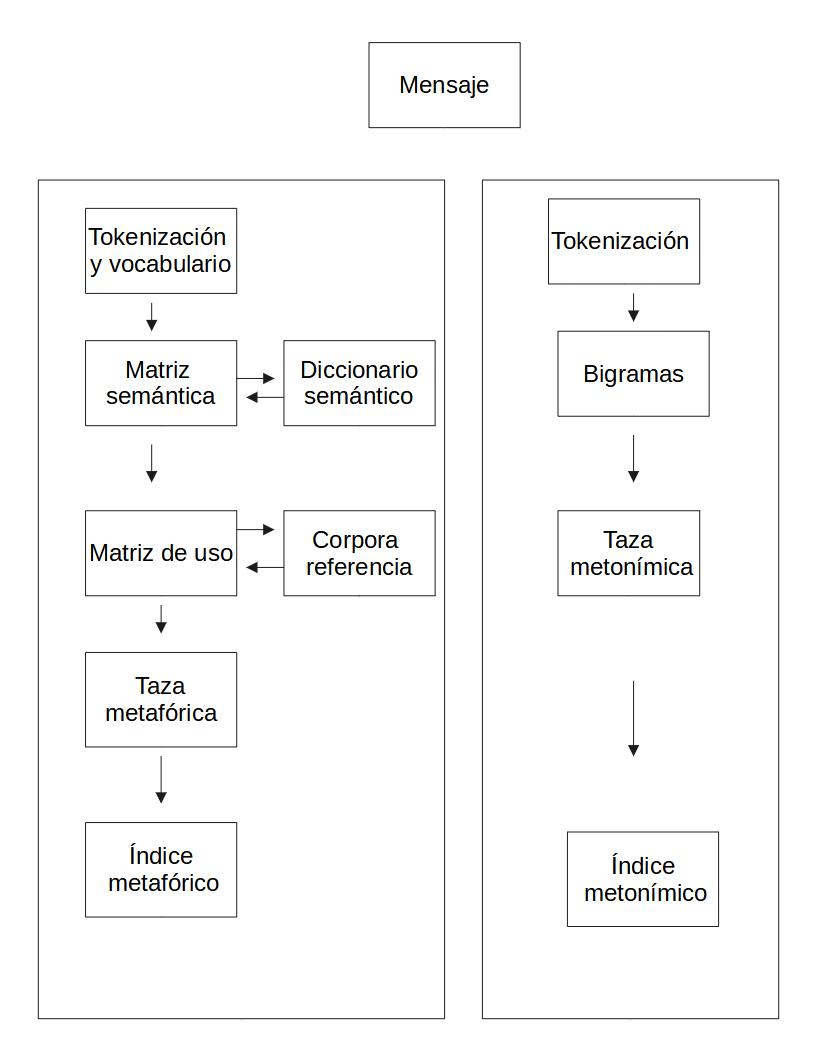
\includegraphics[width=.9\linewidth]{./assets/metodologia.jpg}
\caption{Procesamiento de corpus objetivo}
\end{figure}   
\item Índice Metafórico
\label{sec:orge007d74}
\item Matriz semántica
\label{sec:orgd4522df}


\item Matriz de uso
\label{sec:orge8c016f}

\begin{figure}[htbp]
\centering
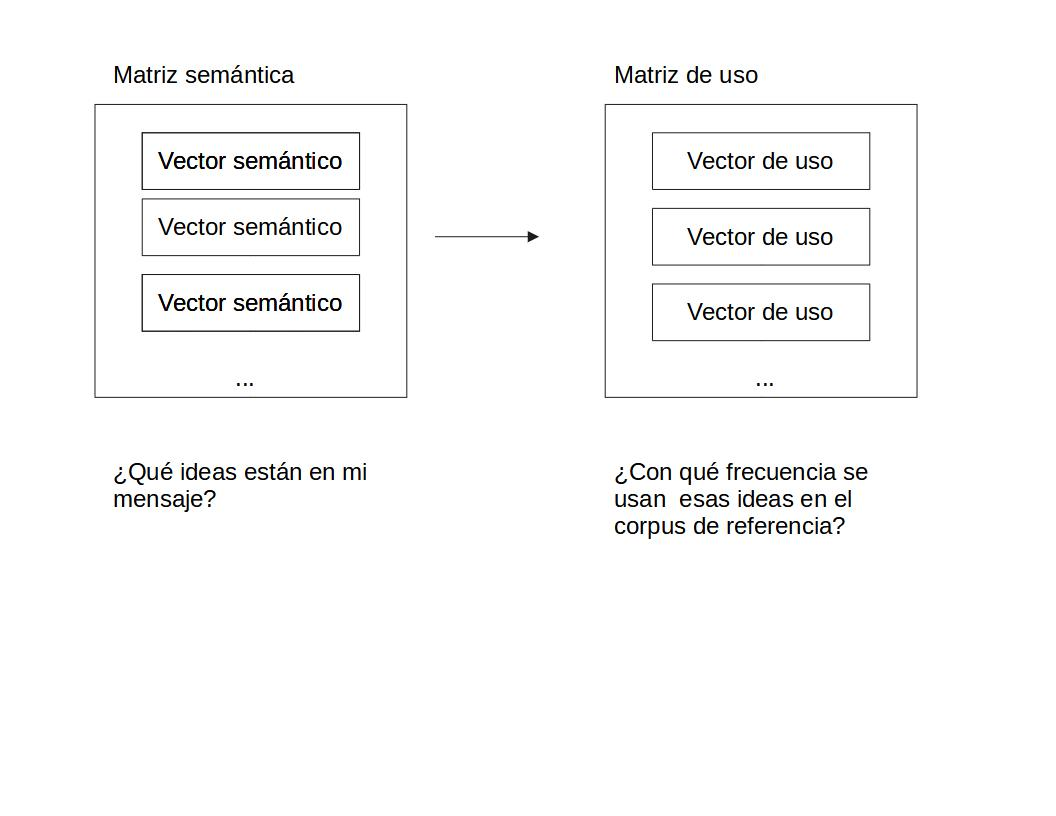
\includegraphics[width=.9\linewidth]{./assets/matrices.jpg}
\caption{Abstracciones necesarias para el índice metafórico}
\end{figure}

\item Índice Metonímico
\label{sec:org4768ba8}
\begin{figure}[htbp]
\centering
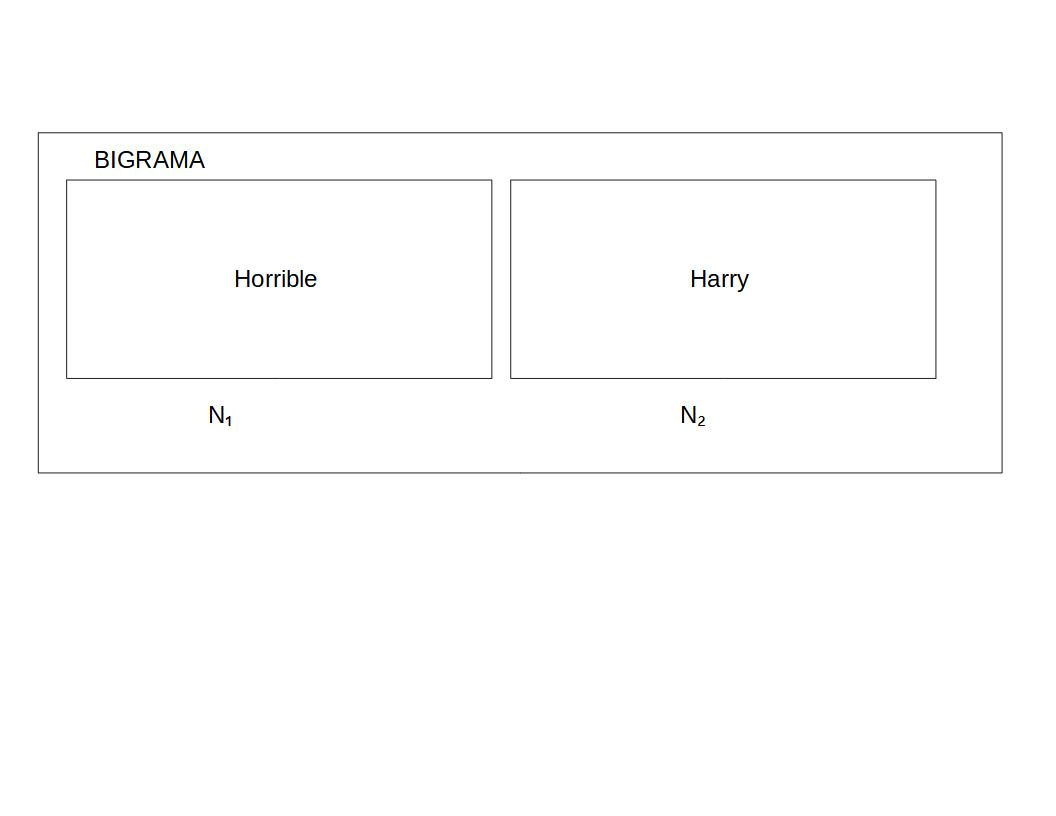
\includegraphics[width=.9\linewidth]{./assets/metonimia.jpg}
\caption{Abstraccciones necesarias para el indice metonímico}
\end{figure}
\end{enumerate}

\subsection{Despliegue (los notebooks?? creo que no hay despliege)}
\label{sec:org5cc149d}

\begin{quote}
Deployment is the process of using your new insights to make
improvements within your organization. This can mean a formal
integration such as the implementation of a IBM® SPSS® Modeler model
producing churn scores that are then read into a data
warehouse. Alternatively, deployment can mean that you use the
insights gained from data mining to elicit change in your
organization. For example, perhaps you discovered alarming patterns in
your data indicating a shift in behavior for customers over the age
of 30. These results may not be formally integrated into your
information systems, but they will undoubtedly be useful for planning
and making marketing decisions.
\end{quote}


       \begin{table}[!ht]
    \centering
    \begin{tabular}{|l|l|l|}
    \hline
        categoria & índice metafórico & w \\ \hline
        reportage & 7524.541176398631 & 2340 \\ \hline
        editorial & 7273.001005175399 & 2262 \\ \hline
        reviews & 7253.977846579716 & 2370 \\ \hline
        religion & 6454.547716937541 & 2314 \\ \hline
        skills \& hobbies & 6177.00807941614 & 2232 \\ \hline
        popular lore & 6369.248078015795 & 2222 \\ \hline
        belles lettres & 6958.927634792041 & 2288 \\ \hline
        miscellaneous & 7255.178115968617 & 2214 \\ \hline
        learned & 4137.726478820393 & 2254 \\ \hline
        general fiction & 6898.164190465642 & 2264 \\ \hline
        mistery and detective fiction & 5882.878135583104 & 2446 \\ \hline
        science fiction & 6763.667294465371 & 2412 \\ \hline
        adventure and western fiction & 5208.702749914055 & 2560 \\ \hline
        romance and love story & 7068.521208726773 & 2428 \\ \hline
    \end{tabular}
\caption{Resultado índice metafórico}
\label{tab:resultado_indice_metaforico}
\end{table}


\section{CONCLUSIONES (Creo que esto se solapa con lo que crisp-dm llama despliege)}
\label{sec:org3bcdd54}



\bibliographystyle{unsrt}
\bibliography{biblio} 
\end{document}